\chapter{具体需求}
  \section{功能需求}
    \subsection{R.FUNC.BB.001 用户登陆}
    \subsubsection{介绍}
    用户在IOS、Android、Web Browse输入账号和密码登录对应账户。登录成功后自动与服务器同步用户数据。
    \subsubsection{输入}
    用户输入邮箱或学号信息与密码,点击登陆。
    \subsubsection{处理和输出}
    \begin{itemize}
      \item 客户端联网查询账号与密码是否匹配,匹配成功完成登录。
      \item 登录成功后,进行数据同步。
      \item 若不匹配则提醒不匹配,请重新输入。
      \item 密码为空,提示密码不得为空
      \item 账户格式错误,提示请输出正确的账号
      \item 连接超时,提示请检查网络连接
    \end{itemize}

\subsection{R.FUNC.BB.002 作业/实验查询}
      \subsubsection{介绍}
      作业/实验查询用于查询作业/实验情况。学生可以查到本人相关课程的作业情况。教师可以查询相应班级所有学生每次作业的提交情况。教学管理人员可以查询到自己所负责所有学生相应的作业提交情况。
      \subsubsection{输入}
      不同用户的输入如下:
      \begin{center}\begin{description}
        \item[学生] 学生的输入为选择响应的课程或总体...
        \item[老师] 老师可以选择相应的班级和某次作业或全部作业...
        \item[教秘] 教秘可以可以选择自己所负责范围内的所有学生和课程的相应信息
      \end{description}\end{center}
      \subsubsection{处理}
      \begin{enumerate}
        \item 连接服务器,检查查询相应的权限,查询数据库。
        \item 连接查询失败,提示超时,并提示用户检查网络或重试。
        \item 连接查询成功,更新本地数据。
      \end{enumerate}
      \subsubsection{输出}
      \begin{itemize}
        \item 显示更新后的本地数据或显示从服务器返回的数据。
        \item 学生端更新相应的日程。
      \end{itemize}

    \subsection{R.FUNC.BB.003 作业/实验/通知发布}
      \subsubsection{介绍}
      作业/实验/通知发布仅供教师端和管理人员使用。可以用于教师发布自己负责课程相关的作业、实验或通知。
      \subsubsection{输入}
      发布首先要新建条目(某次作业或通知等),之后输入相应发布的信息。\\
      输入数据内容如下:
      \begin{itemize}
        \item 作业/实验/通知的名称。
        \item 作业/实验/通知的文本内容。
        \item 学生提交的截至日期,以日历形式选择。
        \item 相应作业的材料,选择上传按键,上传相应文件。
      \end{itemize}
      \subsubsection{处理}
      \begin{enumerate}
        \item 连接服务器,检查查询相应的权限。
        \item 连接失败或权限不对,提示用户。
        \item 连接成功且权限正确,将数据更新到后台数据库中,将文件保存在服务器中。
      \end{enumerate}
      \subsubsection{输出}
      相关数据存入服务器,客户端提示发布成功或其他异常信息。

    \subsection{R.FUNC.BB.004 作业/实验/通知修改删除}
      \subsubsection{介绍}
      仅供教师和管理人员使用。用于修改或删除已发布的作业/实验/通知。
      \subsubsection{输入}
	    \begin{itemize}
        \item 输入为准备修改的作业等的名称。进入发布界面后,输入要修改的内容或选择删除该作业、通知等。
	      \item 若选择发布实验,则需要选择单人完成还是团队完成(实验可用git进行版本控制)。
      \end{itemize}
      \subsubsection{处理}
      \begin{enumerate}
        \item 连接服务器,检查查询相应的权限。
        \item 连接失败或权限不对,提示用户。
        \item 连接成功且权限正确,将数据更新到后台数据库中,将文件保存在服务器中。
      \end{enumerate}
      \subsubsection{输出}
      在客户端上显示更新后的结果。

    \subsection{R.FUNC.BB.005 作业/实验/通知提交}
      \subsubsection{介绍}
      仅供学生使用。学生提交完成的作业、实验或需要提交材料的通知。
      \subsubsection{输入}
      首先学生选择本人准备提交的作业。提交的内容可以如下:
      \begin{itemize}
        \item 作业/实验/通知的文本内容。
        \item 相应的材料,选择上传按键,上传相应文件。
	   \item 通过git提交,需指定要提交的库。
      \end{itemize}
      \subsubsection{处理}
      \begin{enumerate}
        \item 连接服务器
        \item 连接失败,提示超时,并提示用户检查网络或重试。
        \item 若连接成功,检测当前日期与该作业截止日期。
        \item 若已过作业截止日期,则提交失败。
        \item 若未到作业截至时间,上传数据到服务器,返回状态。
        \item 从服务器返回成功,提示上传成功。
        \item 从服务器返回失败,提示用户上传失败。
      \end{enumerate}
      \subsubsection{输出}
      \begin{itemize}
        \item 上传成功与否的提示
        \item 上传成功则作业完成状况标示为已完成,并更新相应的日程。
      \end{itemize}

    \subsection{R.FUNC.BB.006 作业/实验查看与批改}
      \subsubsection{介绍}
      仅供教师端使用。作业/实验查看与批改用与教师查看学生相应的作业或实验。
      \subsubsection{输入}
      \begin{itemize}
        \item 教师选择相应的作业,可选择将本次作业全部下载到本地或在线查看。
        \item 教师选择要查看/批改作业学生的名称或学号。
      \end{itemize}
	    \subsubsection{处理}
      \begin{enumerate}
        \item 检查相应的权限。
        \item 对要查询的作业进行查重。
        \item 将相应数据发送至客户端。
      \end{enumerate}
	    \subsubsection{输出}
      \begin{itemize}
        \item 客户端可看到学生的作业,及作业重复率比较高的同学名单。
        \item 教师可对学生作业进行批改,进入成绩录入的部分。
      \end{itemize}

    \subsection{R.FUNC.BB.007 成绩录入}
      \subsubsection{介绍}
      成绩输入仅供教师端使用。可以用于登记考试/作业等等的成绩。
      \subsubsection{输入}
      输入时首先要新建条目(某次考试或者作业等),之后再相应的输入各学生成绩数据。输入有以下几种方式:
      \begin{itemize}
        \item 从文件中读取输入,系统支持从文件中导入成绩,具体导入格式如下所示
        \begin{lstlisting}[caption=文件导入成绩示例, label={code:import_grade_from_file}]
        #学号,成绩以','分隔,每行一条记录。
        #例:
        张三,96
        李四,90
        \end{lstlisting}
        \item 通过客户端逐条进行输入
        \item 导入作业批改系统自动生成的成绩
      \end{itemize}
      输入数据要求如下:
      \begin{itemize}
        \item 学号必须是登记注册为本课程的学生的有效学号,否则进行报错。
        \item 成绩为整数,如果含有小数按四舍五入进行舍入。
        \item 默认成绩的范围为[0,100],超过此范围进行警告并且自动取最接近的可行值。可以通过自定义设置进行调整。
      \end{itemize}
    \subsubsection{处理}
    \begin{enumerate}
      \item 按照默认规则和用户自定义的规则生成相关的约束对于输入数据的有效性进行验证。如果含有出错首先按照默认处理逻辑处理并且给出警告.
      \item 如果不存在适配的处理流程则报错并要求用户进行修改。
      \item 如果所有验证有效,转换为指定格式存入相应的后台数据库中。
    \end{enumerate}
    \subsubsection{输出}
    数据最终存入后端的数据库中。

  \subsection{R.FUNC.BB.008 成绩查询}
    \subsubsection{介绍}
    成绩查询用于查询已经录入的成绩。学生可以查到本人相应课程的所有成绩。老师可以查到相应班级所有同学的成绩。教学管理人员可以查询自己所负责所有学生的相应成绩。
    \subsubsection{输入}
    不同用户的输入如下:
    \begin{center}\begin{description}
      \item[学生] 学生的输入为选择响应的课程和某次考试/作业/...
      \item[老师] 老师可以选择相应的班级和某次考试/作业/...
      \item[教秘] 教秘可以可以选择自己所负责范围内的所有学生和课程的相应信息
    \end{description}\end{center}
    \subsubsection{处理}
    \begin{enumerate}
      \item 消息传递给后端数据库后检查相应的权限
      \item 权限不足给出警告
      \item 权限符合则取出相应的数据传回
    \end{enumerate}
    \subsubsection{输出}
    接受后端数据库传回的数据并显示在客户端上。

  \subsection{R.FUNC.BB.009 成绩统计和调整}
    \subsubsection{介绍}
    成绩统计功能教学管理人员与老师都拥有,成绩调整只有老师有相应的权限。成绩统计可用于老师和教学管理人员了解教学情况以及学生的学业状况。成绩调整可以供老师修订成绩同时也可以方便按照一定的规则对于成绩进行统一调整使得成绩更有一般性并能更好的体现学生的水平。预置部分功能如下:
    \begin{description}
      \item[统计] 可以进行求和、平均、排序等等基本操作
      \item[修改] 可以按照预置或者自定义的一些规则对成绩进行统一调整,如正态话等等
    \end{description}
    \subsubsection{输入}
    输入选择操作成绩的对象。对象的约束包括学生和哪次考试两方面。同时需要指定相应的数据操作。
    \subsubsection{处理}
    根据输入操作对象,首先检查用户是否具有相应的权限,然后从后台数据库中取出相应的数据。按照输入中指定的操作进行处理。输出时询问用户是否要同时更新数据库中内容。
    \subsubsection{输出}
    在客户端中显示结果,同时根据操作类型和用户的选择决定是否需要更新原数据库。

  \subsection{R.FUNC.BB.010 资源上传}
    \subsubsection{介绍}
    资源上传可用于教师分享课件等教学辅助材料。同时同学自身也可以分享有用材料。空间分为共享和私有两部分。私有空间可以用作个人文件的托管和同步。
    \subsubsection{输入}
    输入给定指定资源来源以及上传目的地,源有以下选项:
    \begin{itemize}
      \item 从本地进行上传
      \item 给出相应的下载链接进行离线下载
      \item 从别人共享文件处进行同步
    \end{itemize}
    目的地有以下选项:
    \begin{itemize}
      \item 私人拥有的库,但是可以设置是否他人可见
      \item 共享资源库中,需要检查权限,无权限者需要经过管理员审核。默认上传之后会对所有相关人员广播通知。共享资源库可以由个人建立之后邀请相关人员加入。每门课程建立之后会生成相应课程资源区,老师助教拥有权限并且加入相应的学生。同时各行政院系等也会有相应打资源共享区。
    \end{itemize}
    同时还要给出资源相应的权限设置如是否共享以及是否通知他人等。
    \subsubsection{处理}
    \begin{enumerate}
      \item 对于给定的输入,首先判断对于目的地是否具有相应的权限,如无报错,如果需要申请先进行请求。有或者请求通过则继续。
      \item 然后检查相应的资源是否有效合法。如验证有效则快速比较后台数据库是否已经存在相应的数据,如不存在则存储,否则只建立相应的链接。
    \end{enumerate}
    \subsubsection{输出}
    将数据实际存储入相应服务器,同时反馈操作结果。

  \subsection{R.FUNC.BB.012 资源下载与浏览}
    \subsubsection{介绍}
    资源下载用于获取远端分享的相关资源
    \subsubsection{输入}
    请求的资源以及请求的操作
    \subsubsection{处理}
    \begin{enumerate}
      \item 检查响应的请求是否具有相关的权限,如果是下载则后台开启传输。
      \item 如果是浏览则尝试进行打开。
    \end{enumerate}
    暂时支持浏览的文件类型如下:
    \begin{itemize}
      \item
    \end{itemize}
    \subsubsection{输出}
    下载存储至本地,浏览输出至相应的客户端。

  \subsection{R.FUNC.BB.013 新建日程}
    \subsubsection{介绍}
    本功能用于生成新的日程安排,辅助用户合理安排各项任务
    \subsubsection{输入}
    新建日程主要可以通过以下几种方式:
    \begin{itemize}
      \item 直接由用户输入各项参数生成新的日程提醒
      \item 通过作业实验以及考试等的通知安排自动生成日程
      \item 用户直接复制收到的通知等文本,提取其中的信息自动生成相关的日程
    \end{itemize}
    每项日程有以下参数构成:
    \begin{itemize}
      \item 事件开始时间和结束时间,如果开始时间和结束时间相同则将此时间视作截止时间
      \item 事件的地点
      \item 事件简要说明
      \item 事件的详细说明,可链接至相应备忘/作业/实验/...处
      \item 提醒时间,可自定义多个,缺省在开始前一天以及前一个小时进行提醒
      \item 其他自定义标签
    \end{itemize}
    \subsubsection{处理}
    处理流程如下:
    \begin{enumerate}
      \item 首先对输入进行解析,从中提取出相应的各项参数信息
      \item 对信息进行分析,检查是否有不合法之处,如当前时间已超出截止时间,该时间段已经有其他安排等并给出相应的提醒
      \item 根据信息生成日程安排存储至后端数据库并生成相应的提醒
    \end{enumerate}
    \subsubsection{输出}
    输出一是存储至本地数据库中同时同步至远端,另外反馈是否成功。

  \subsection{R.FUNC.BB.014 日程显示与提醒}
    \subsubsection{介绍}
    日程提醒显示用于提醒自身的任务安排,合理安排时间。避免遗忘重要事项。
    \subsubsection{输入}
    数据库中现存的日程数据。
    \subsubsection{处理}
    \begin{enumerate}
      \item 将数据库中存储的日程信息获取
      \item 按用户指定方式排序,按照事件进行排布并输出至客户端。
      \item 用截止日期和当前时间自动计算倒计时。同时检查是否有需要进行提醒的事项
    \end{enumerate}
    \subsubsection{输出}
    输出至客户端相应页面,同时可调用铃声系统通知等进行提醒。

  \subsection{R.FUNC.BB.015 讨论区讨论}
    \subsubsection{介绍}
    讨论区可以发布新的主题用于进行问题讨论,增强对知识的理解和应用。
    讨论区需要具备以下功能:
    \begin{itemize}
      \item 发布新的主题
      \item 回复
      \item 修订
    \end{itemize}
    \subsubsection{输入}
    \begin{itemize}
      \item 所选择的操作:新建主题、回复等等
      \item 操作内容,支持富文本格式
    \end{itemize}
    \subsubsection{处理}
    \begin{enumerate}
      \item 检查是否具有相关权限并简单判断内容是否合法。
      \item 转换为指定的存储格式
      \item 判断是否需要广播该消息以及广播对象。
    \end{enumerate}
    \subsubsection{输出}
    存储至后台数据库中。如果需要广播调用广播接口。

  \subsection{R.FUNC.BB.016 新建博文}
    \subsubsection{介绍}
    博文主要用于用户分享学习经验等等认为有意义的东西,相比讨论区更加系统。
    \subsubsection{输入}
    新建博文的主题以及内容。
    \subsubsection{处理}
    转换为相应的存储结构存储至后台服务器。
    \subsubsection{输出}
    输出存储至后台数据库并反馈是否成功。

  \subsection{R.FUNC.BB.017 课程考试排布}
    \subsubsection{介绍}
    课程考试排布功能主要用于辅助教学管理人员合理安排相关活动,减少冲突节约时间。
    \subsubsection{输入}
    \begin{itemize}
      \item 对象学生的信息
      \item 课程考试相关信息
      \item 其他约束条件
    \end{itemize}
    \subsubsection{处理}
    调用相关算法生成满足一下条件的课表:
    \subsubsection{输出}
    生成的课表信息


 \subsection{R.FUNC.BB.018 学习笔记文本添加}
    \subsubsection{介绍}
    学生用户在课堂或者课下记录笔记。
    \subsubsection{输入}
    用户选择创建新的笔记或者修改已经存在的笔记,进入文本编辑界面进行,编辑完成后点击保存到本地或者上传,点击返回键退出。
    \subsubsection{处理}
    \begin{enumerate}
      \item 记录笔记创建的课程名称。
      \item 记录笔记创建的时间,和最后一次进行编辑的时间。
      \item 点击保存到本地之后,保存笔记内容,并写入本地存储器。
      \item 点击上传,保存笔记内容,上传到服务器。
      \item 点击返回键,不保存返回上一层。
    \end{enumerate}
    \subsubsection{输出}
	  保存已记录的笔记,同步。
  \subsection{R.FUNC.BB.019 学习笔记课件修改}
    \subsubsection{介绍}
	   学生用户在老师上传的课件上使用文本框或者画图功能添加批注笔记。
    \subsubsection{输入}
	   用户在编辑阶段,点击添加画图或文本框。
    \subsubsection{处理}
    \begin{enumerate}
      \item 添加画图,在课件编辑界面进行画图,结束之后保存更改后的课件。
      \item 添加文本框,进入文本编辑界面输入文本框,并插入到课件中用户指定位置上。
    \end{enumerate}
    \subsubsection{输出}
	   用户在课程课件上添加笔记或画图。

 \subsection{R.FUNC.BB.020 学习笔记搜索}
    \subsubsection{介绍}
	   对笔记(文本模块和课件模块)进行检索,可根据创建时间,修改时间,课程,文本进行搜索。
    \subsubsection{输入}
	   用户点击搜索按钮,输入关键字
    \subsubsection{处理和输出}
    \begin{itemize}
      \item 根据用户输入的搜索关键字进行搜索,结果按照时间,课程,文本可选分类显示
      \item 无搜索结果则显示无结果
    \end{itemize}

 \subsection{R.FUNC.BB.021 学习笔记删除}
    \subsubsection{介绍}
	   删除某一笔记
    \subsubsection{输入}
	   用户长按笔记,点击删除按钮,删除云端保存的笔记。
    \subsubsection{处理与输出}
	   对用户点击笔记进行删除,并进行数据同步,输出删除成功。

 \subsection{R.FUNC.BB.022 学习笔记导出}
    \subsubsection{介绍}
	   对用户的文本笔记和做过笔记的课件进行导出。
    \subsubsection{输入}
	   用户点击导出按钮,并选择导出格式和保存目录。
    \subsubsection{处理和输出}
    \begin{enumerate}
      \item 连接服务器,将用户的请求数据处理打包发送到用户端。
      \item 按照制定格式和目录保存。
      \item 若连接服务器超时,则提示超时,重新导出。
    \end{enumerate}

 \subsection{R.FUNC.BB.023 学习笔记共享}
    \subsubsection{介绍}
	   用户与其他用户共享学习笔记。
    \subsubsection{输入}
	   用户勾选想要与同课程下其他用户共享的笔记,点击共享。
    \subsubsection{处理和输出}
    \begin{enumerate}
      \item 连接服务器,更改所选笔记的访问权限,并显示共享成功
      \item 若连接服务器超时,则提示超时,重新共享
    \end{enumerate}

\section{外部接口需求}
  \subsection{用户接口}
  界面支持多尺寸手机屏幕,web端支持使用IE、Safari、chrome、Firefox浏览器。\par
  以IOS界面为例,分为用户登录,日程显示,作业实验查询,讨论区,笔记等部分。
    \subsubsection{R.HW.INTF.BB.001 登录}
    \begin{figure}[H]
    \centering
    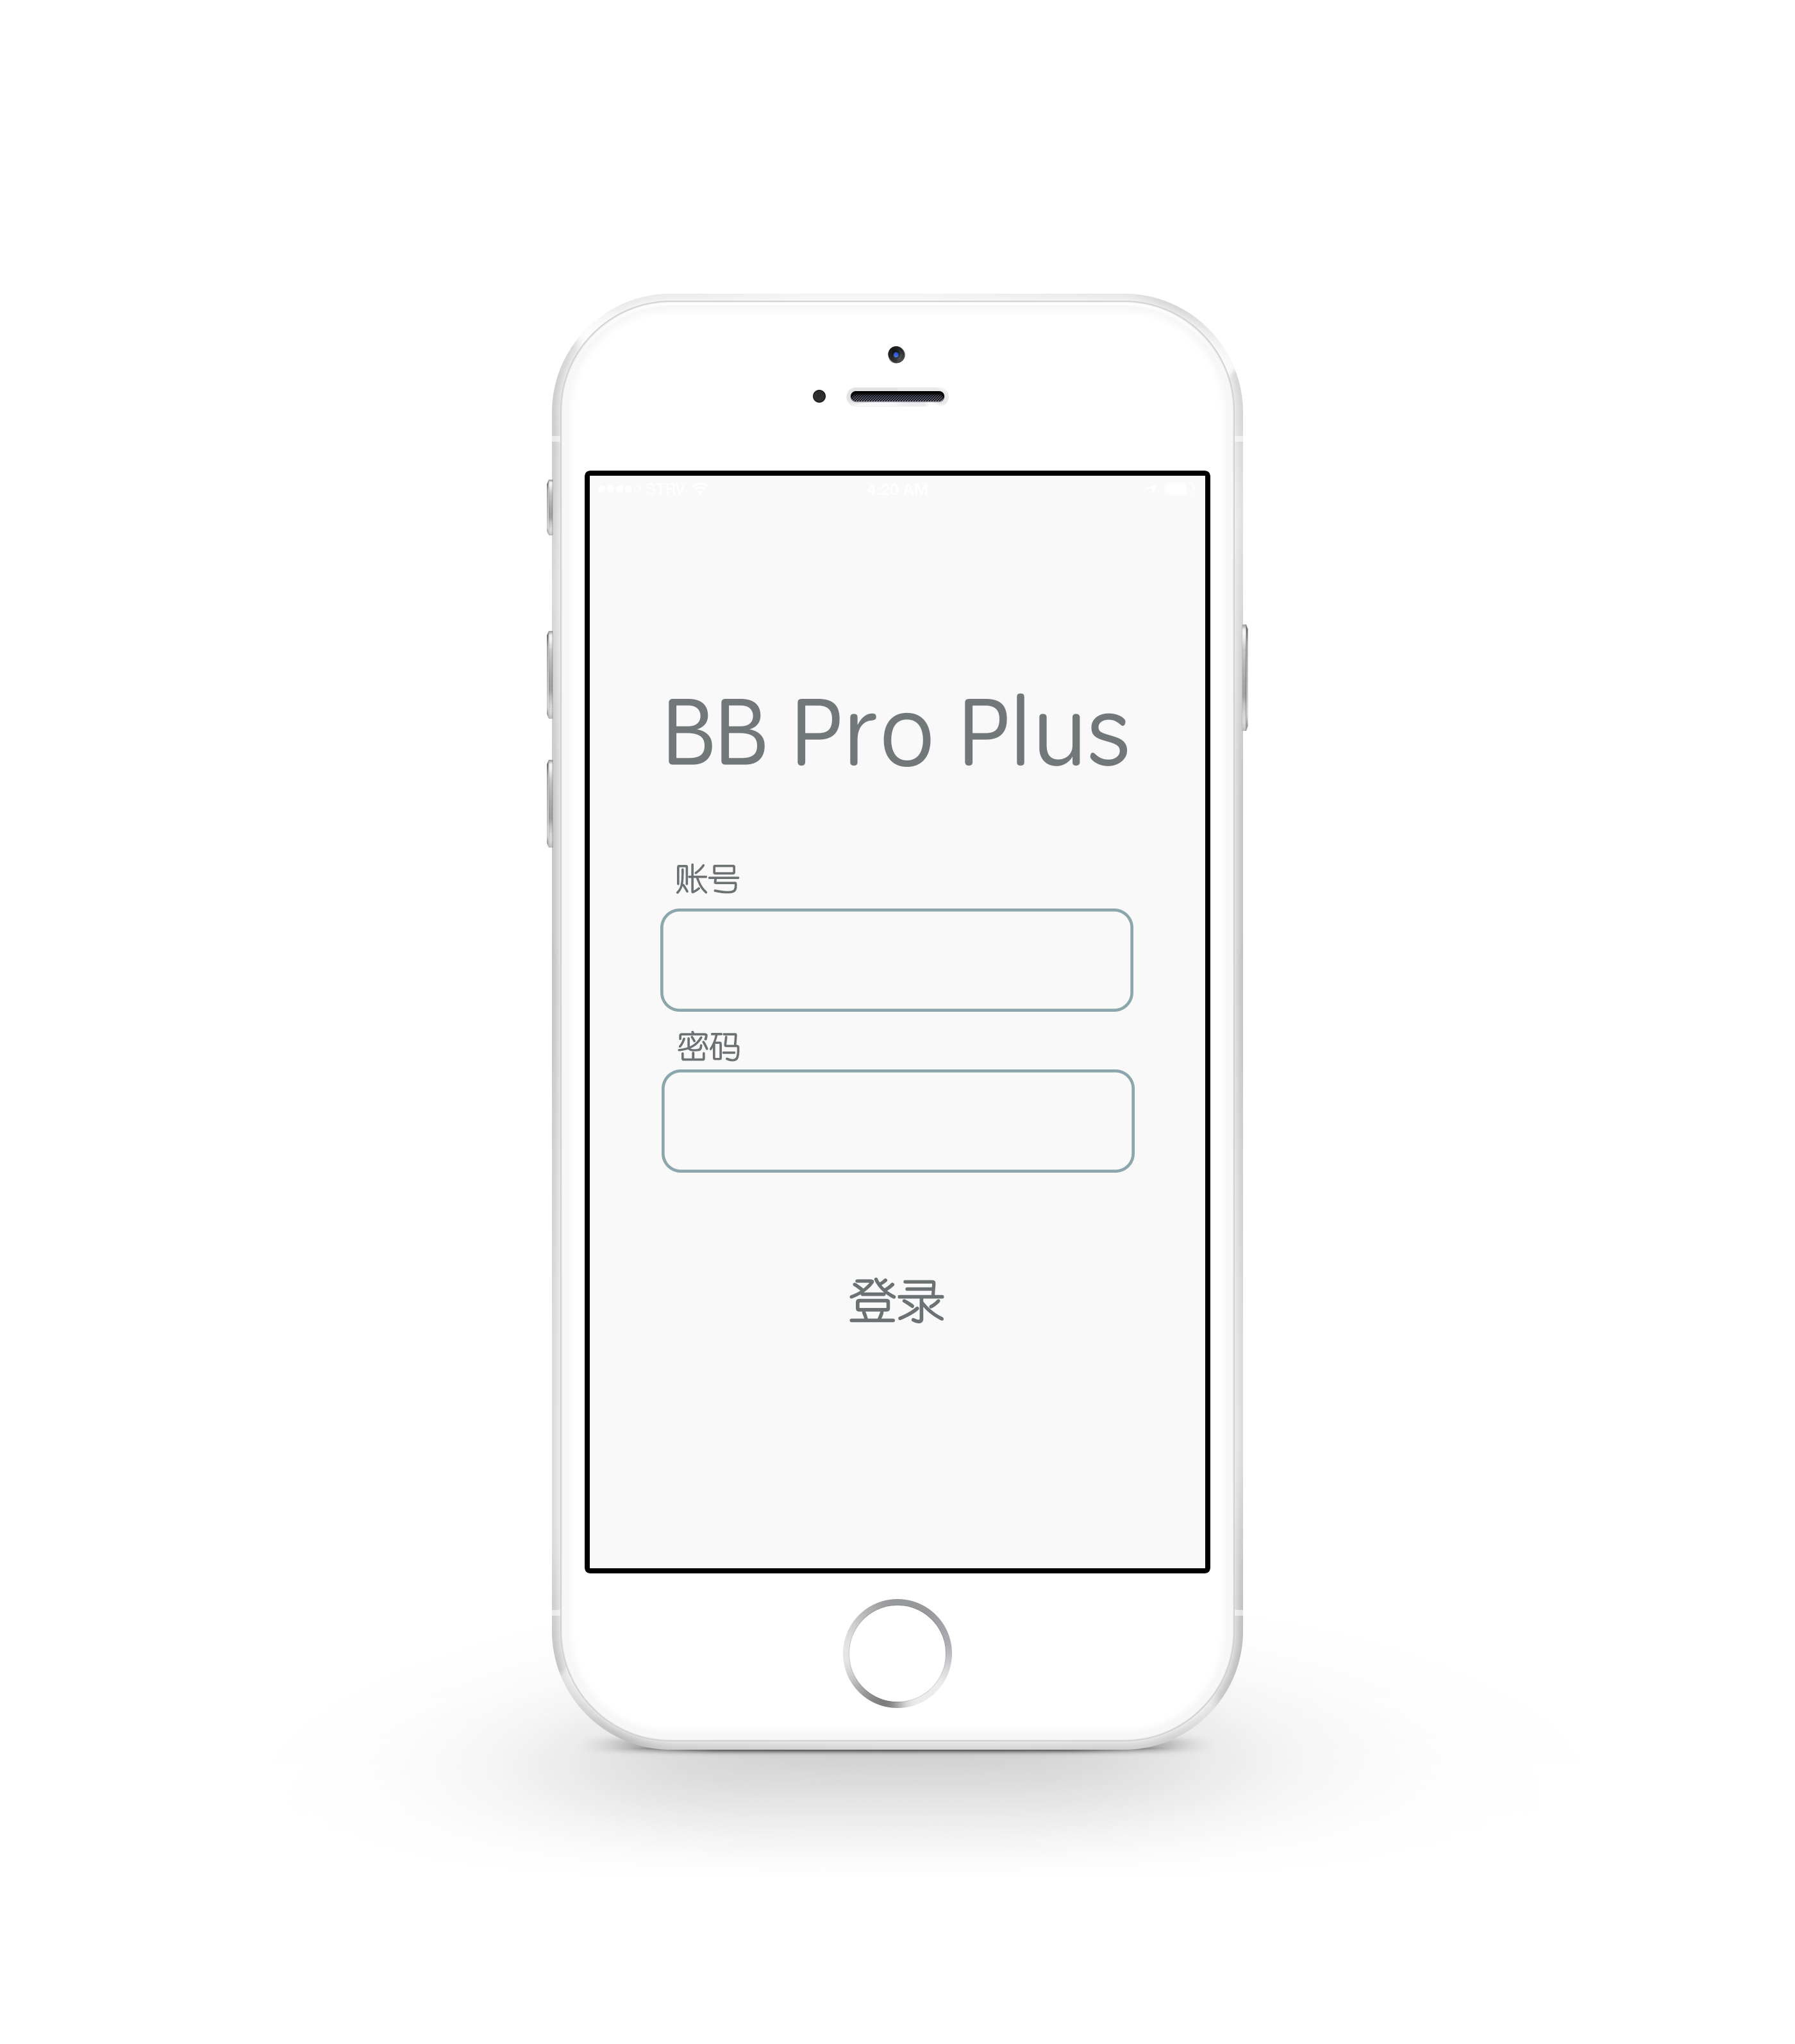
\includegraphics[width=10cm]{login}
    \caption{登陆界面}
    \end{figure}
    \begin{itemize}
      \item 账号:填写科大邮箱或者学号
      \item 密码:填写密码
      \item 登录按钮:点击登录
    \end{itemize}
    \subsubsection{R.HW.INTF.BB.002 日程日历化显示}
    \begin{figure}[H]
    \centering
    \subfigure[日程显示]{
    \begin{minipage}{7cm}
    \centering
    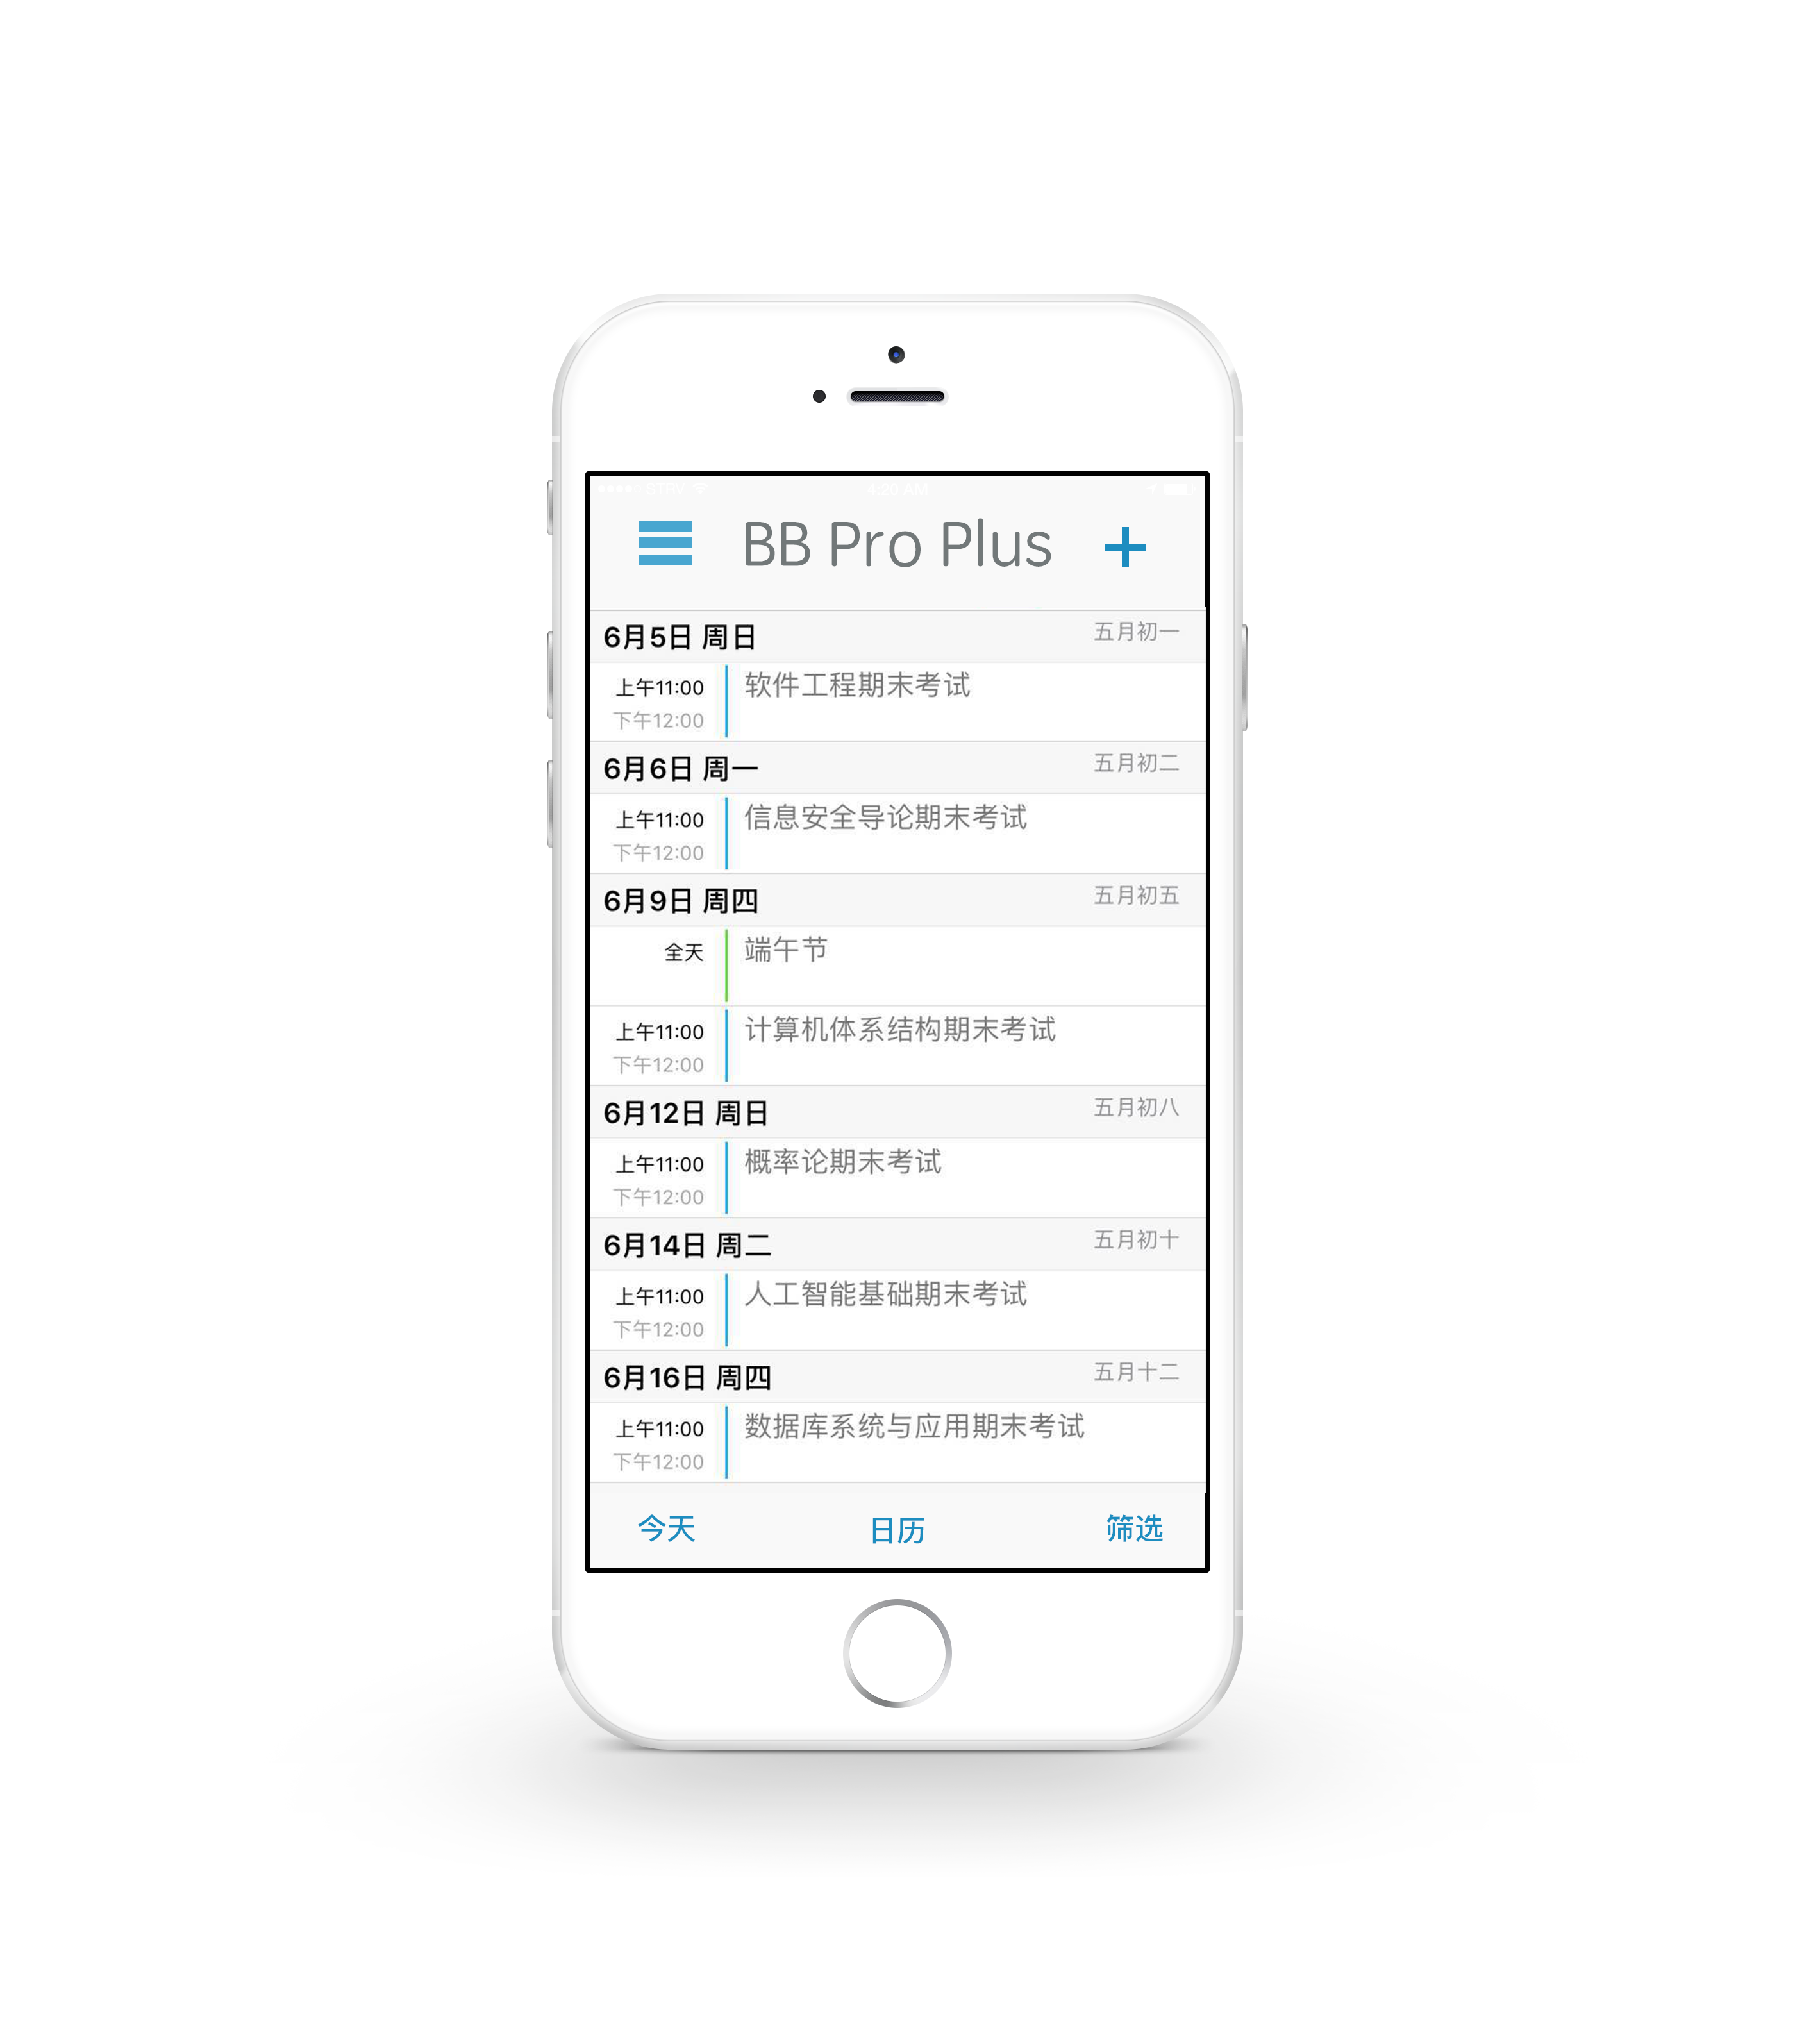
\includegraphics[width=10cm]{ddl}
    \end{minipage}
    }
    \subfigure[菜单栏]{
    \begin{minipage}{7cm}
    \centering
    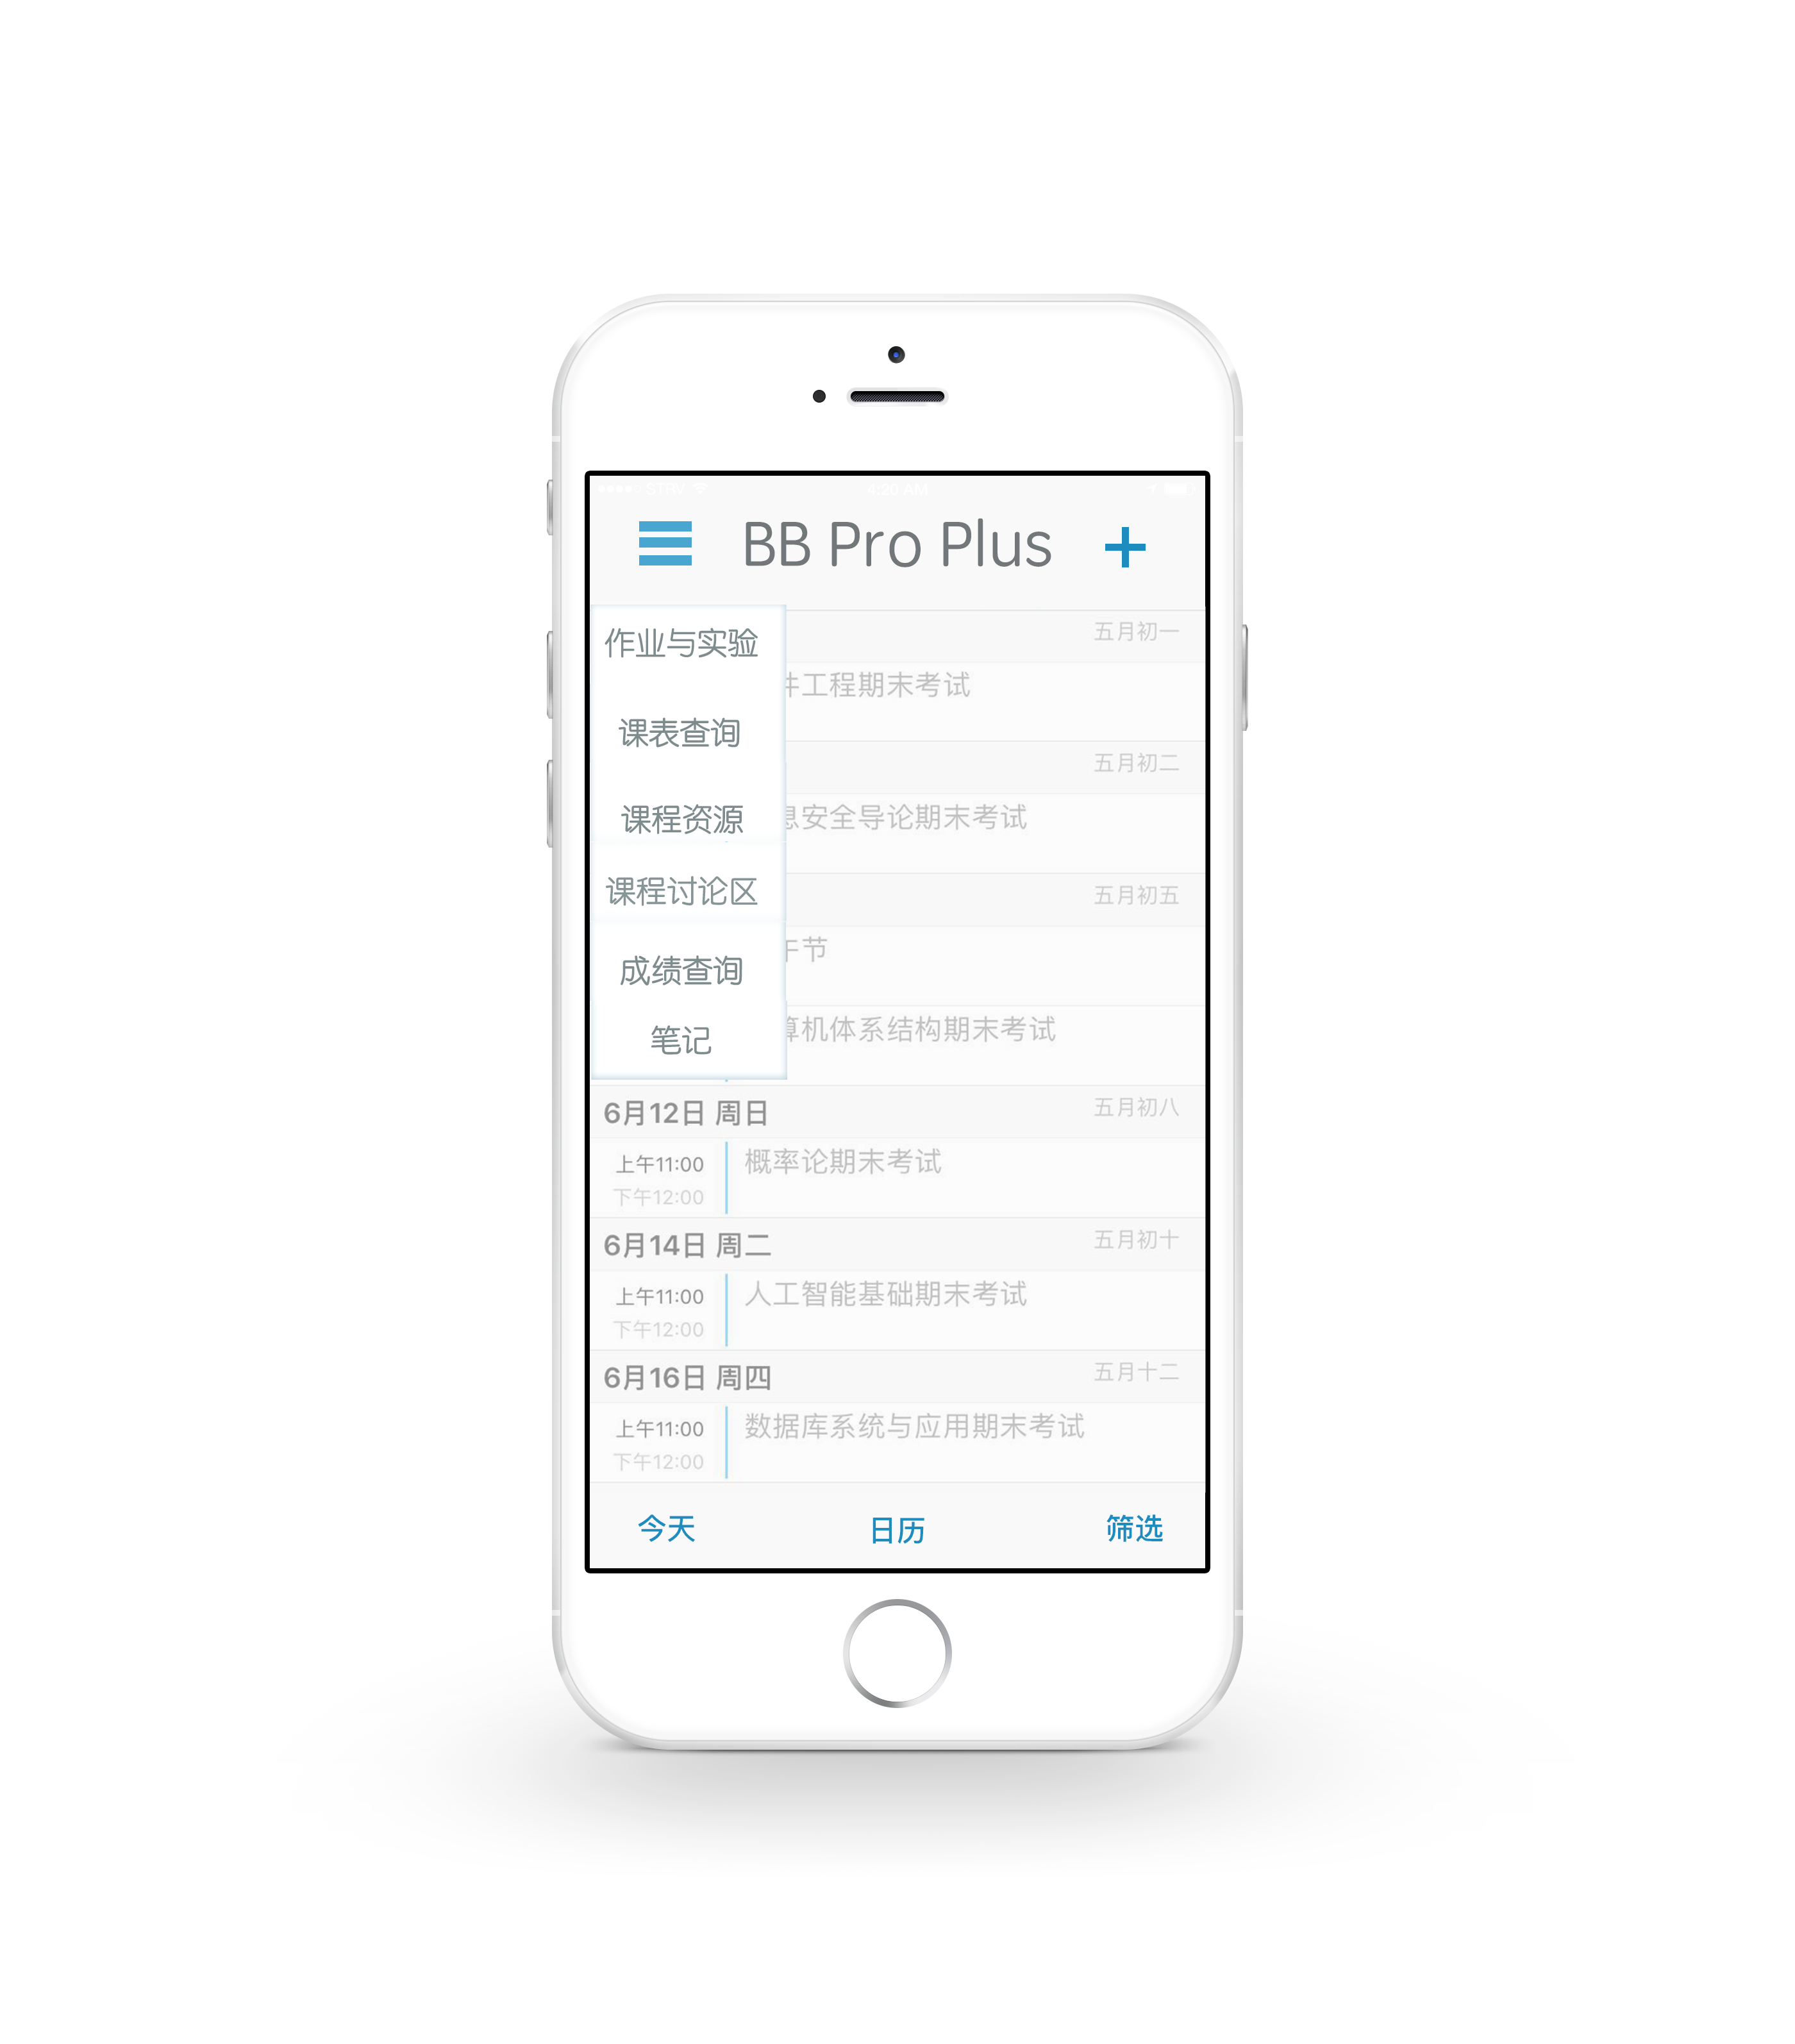
\includegraphics[width=10cm]{menu}
    \end{minipage}
    }
    \caption{}
    \end{figure}
    \begin{itemize}
      \item +按钮:新建日程
      \item 今天:显示今天待提交的实验或作业
      \item 日历:显示日历
      \item 筛选:按指定规则筛选时间
      \item 点击日程标题:进入作业或实验的具体页面
      \item 菜单页面:点击选择功能
    \end{itemize}
    \subsubsection{R.HW.INTF.BB.003 作业实验查询}
    \begin{figure}[H]
    \centering
    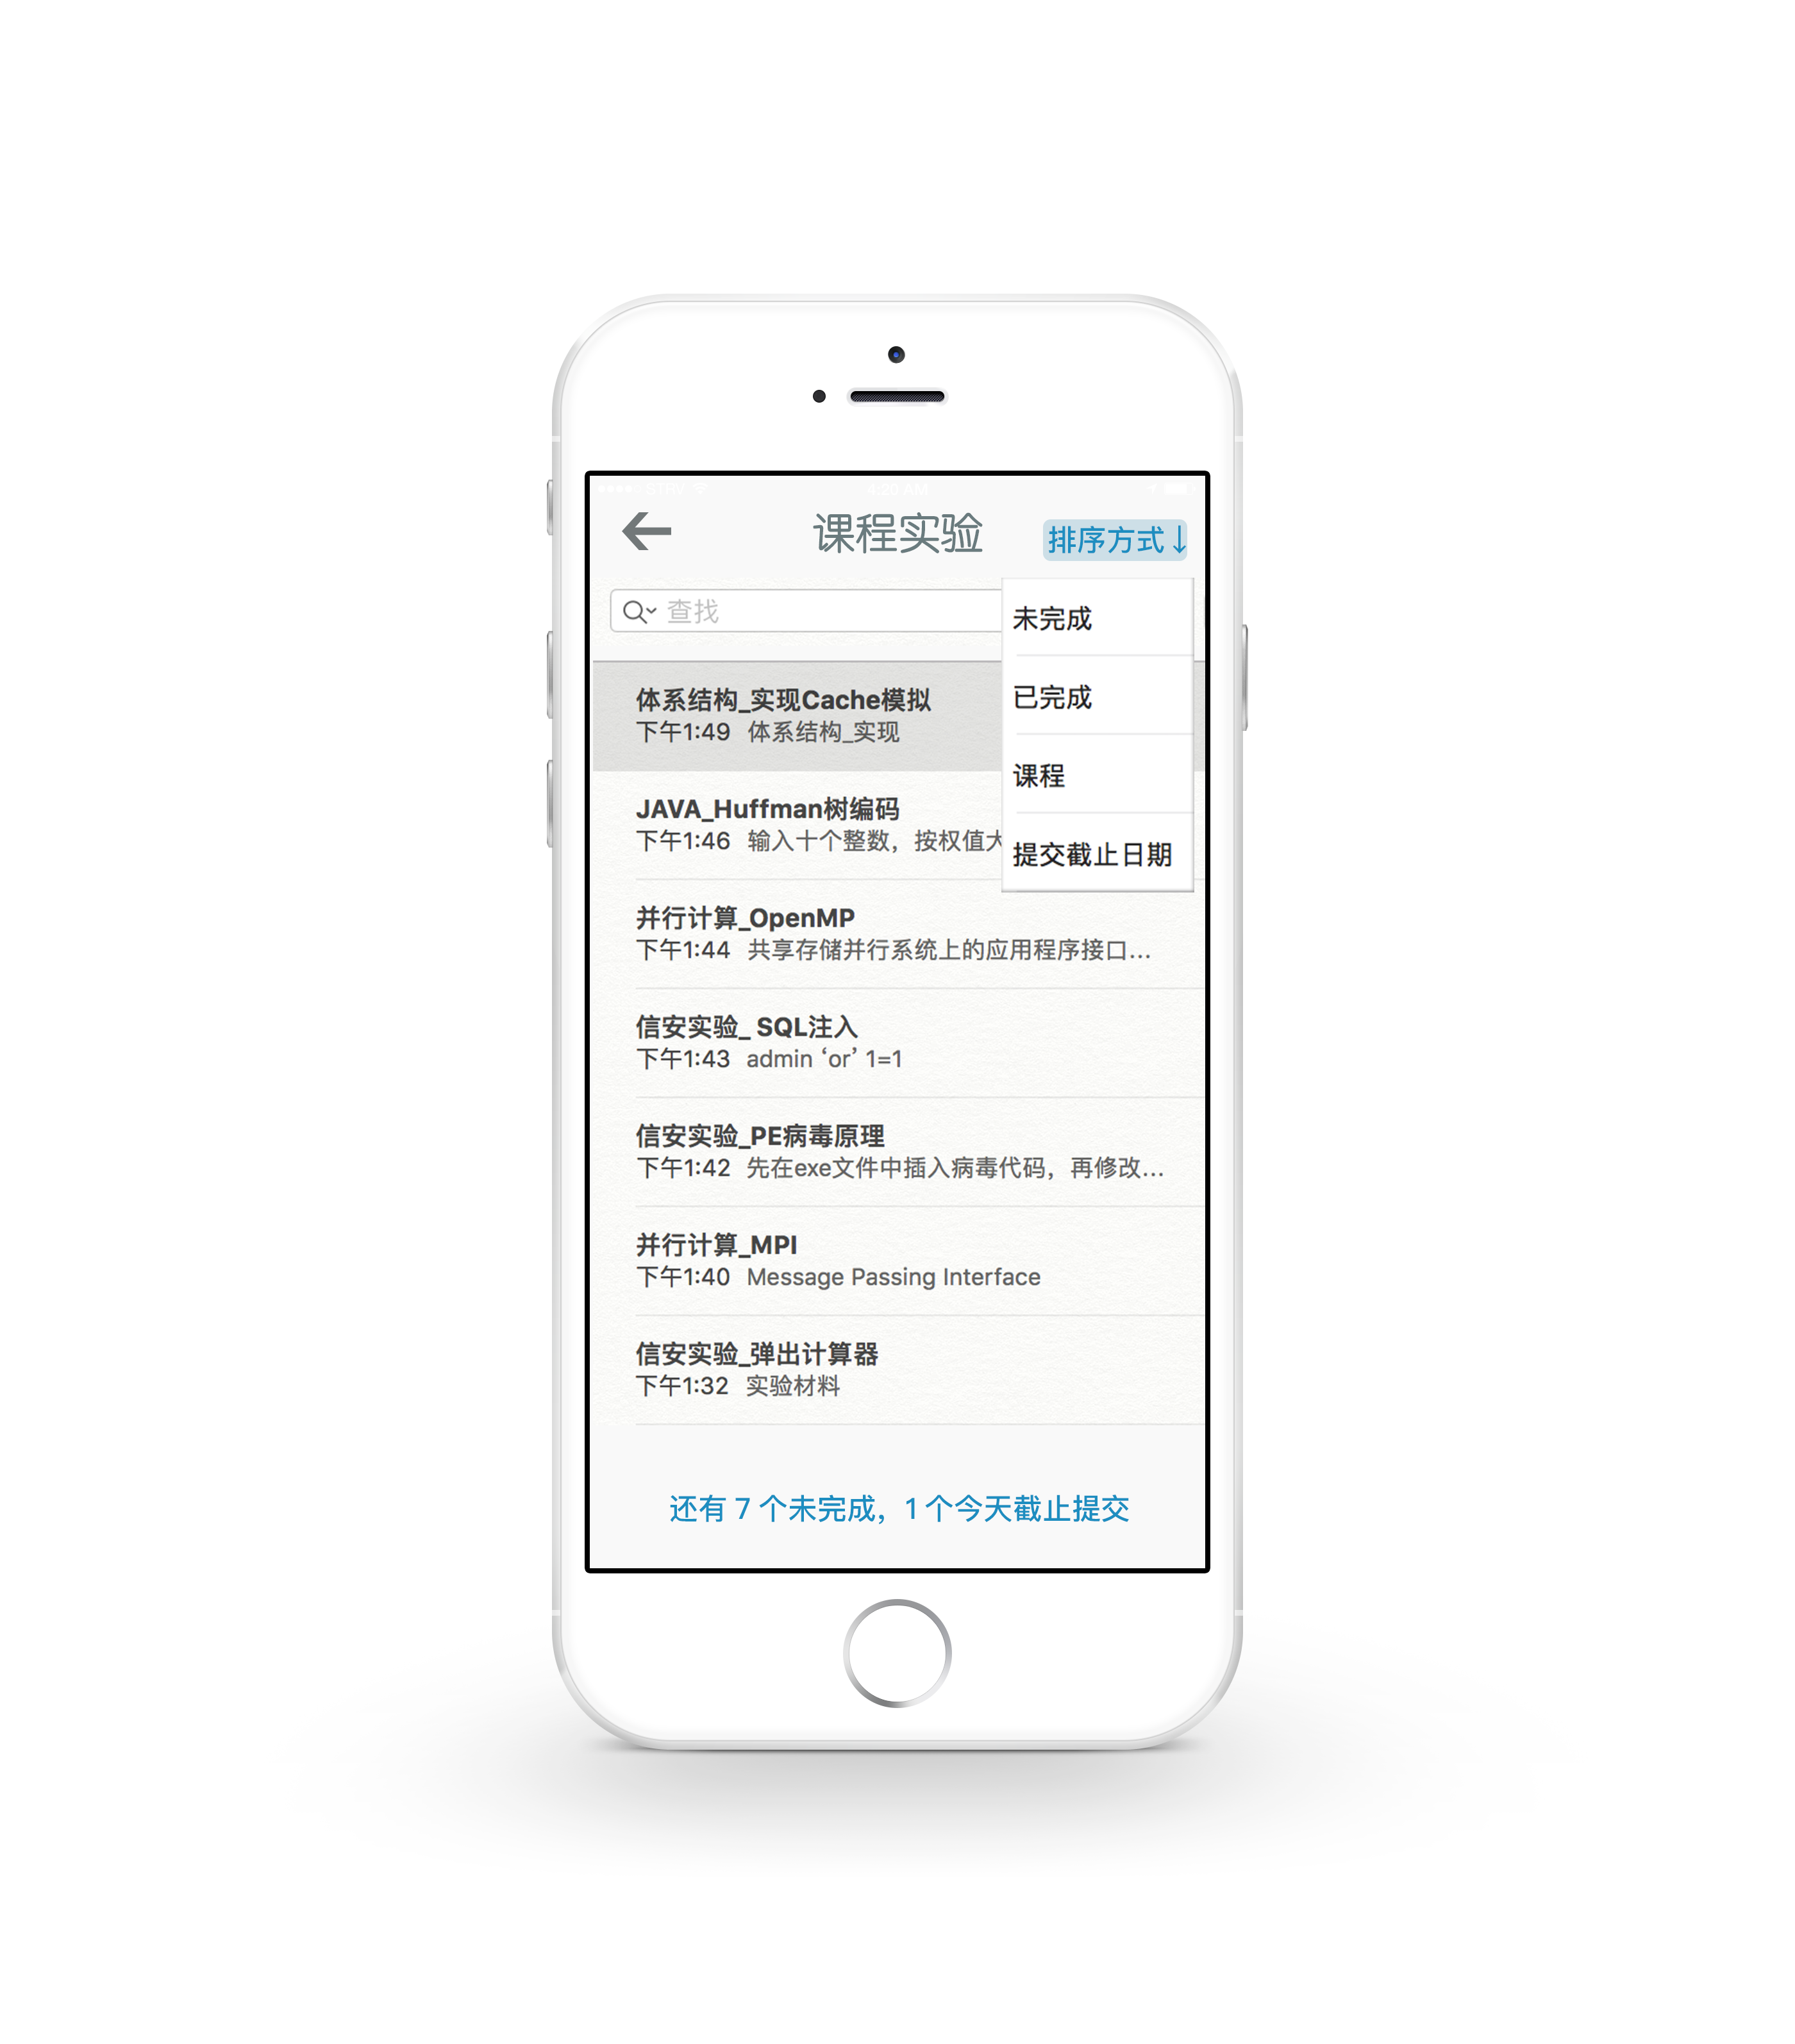
\includegraphics[width=10cm]{experiment_list}
    \caption{实验列表}
    \end{figure}
    \begin{itemize}
  \item  排序方式按钮:选择排序方式
  \item -未完成:显示所有未完成任务
  \item -已完成:显示已完成任务
  \item -课程:按课程分类
  \item -提交截止日期:按截止日期正序排序
  \item 查找框:按用户输入关键词搜索
  \item 点击标题:进入作业或实验的具体页面
  \item 菜单按钮:查看功能菜单
  \begin{figure}[H]
  \centering
  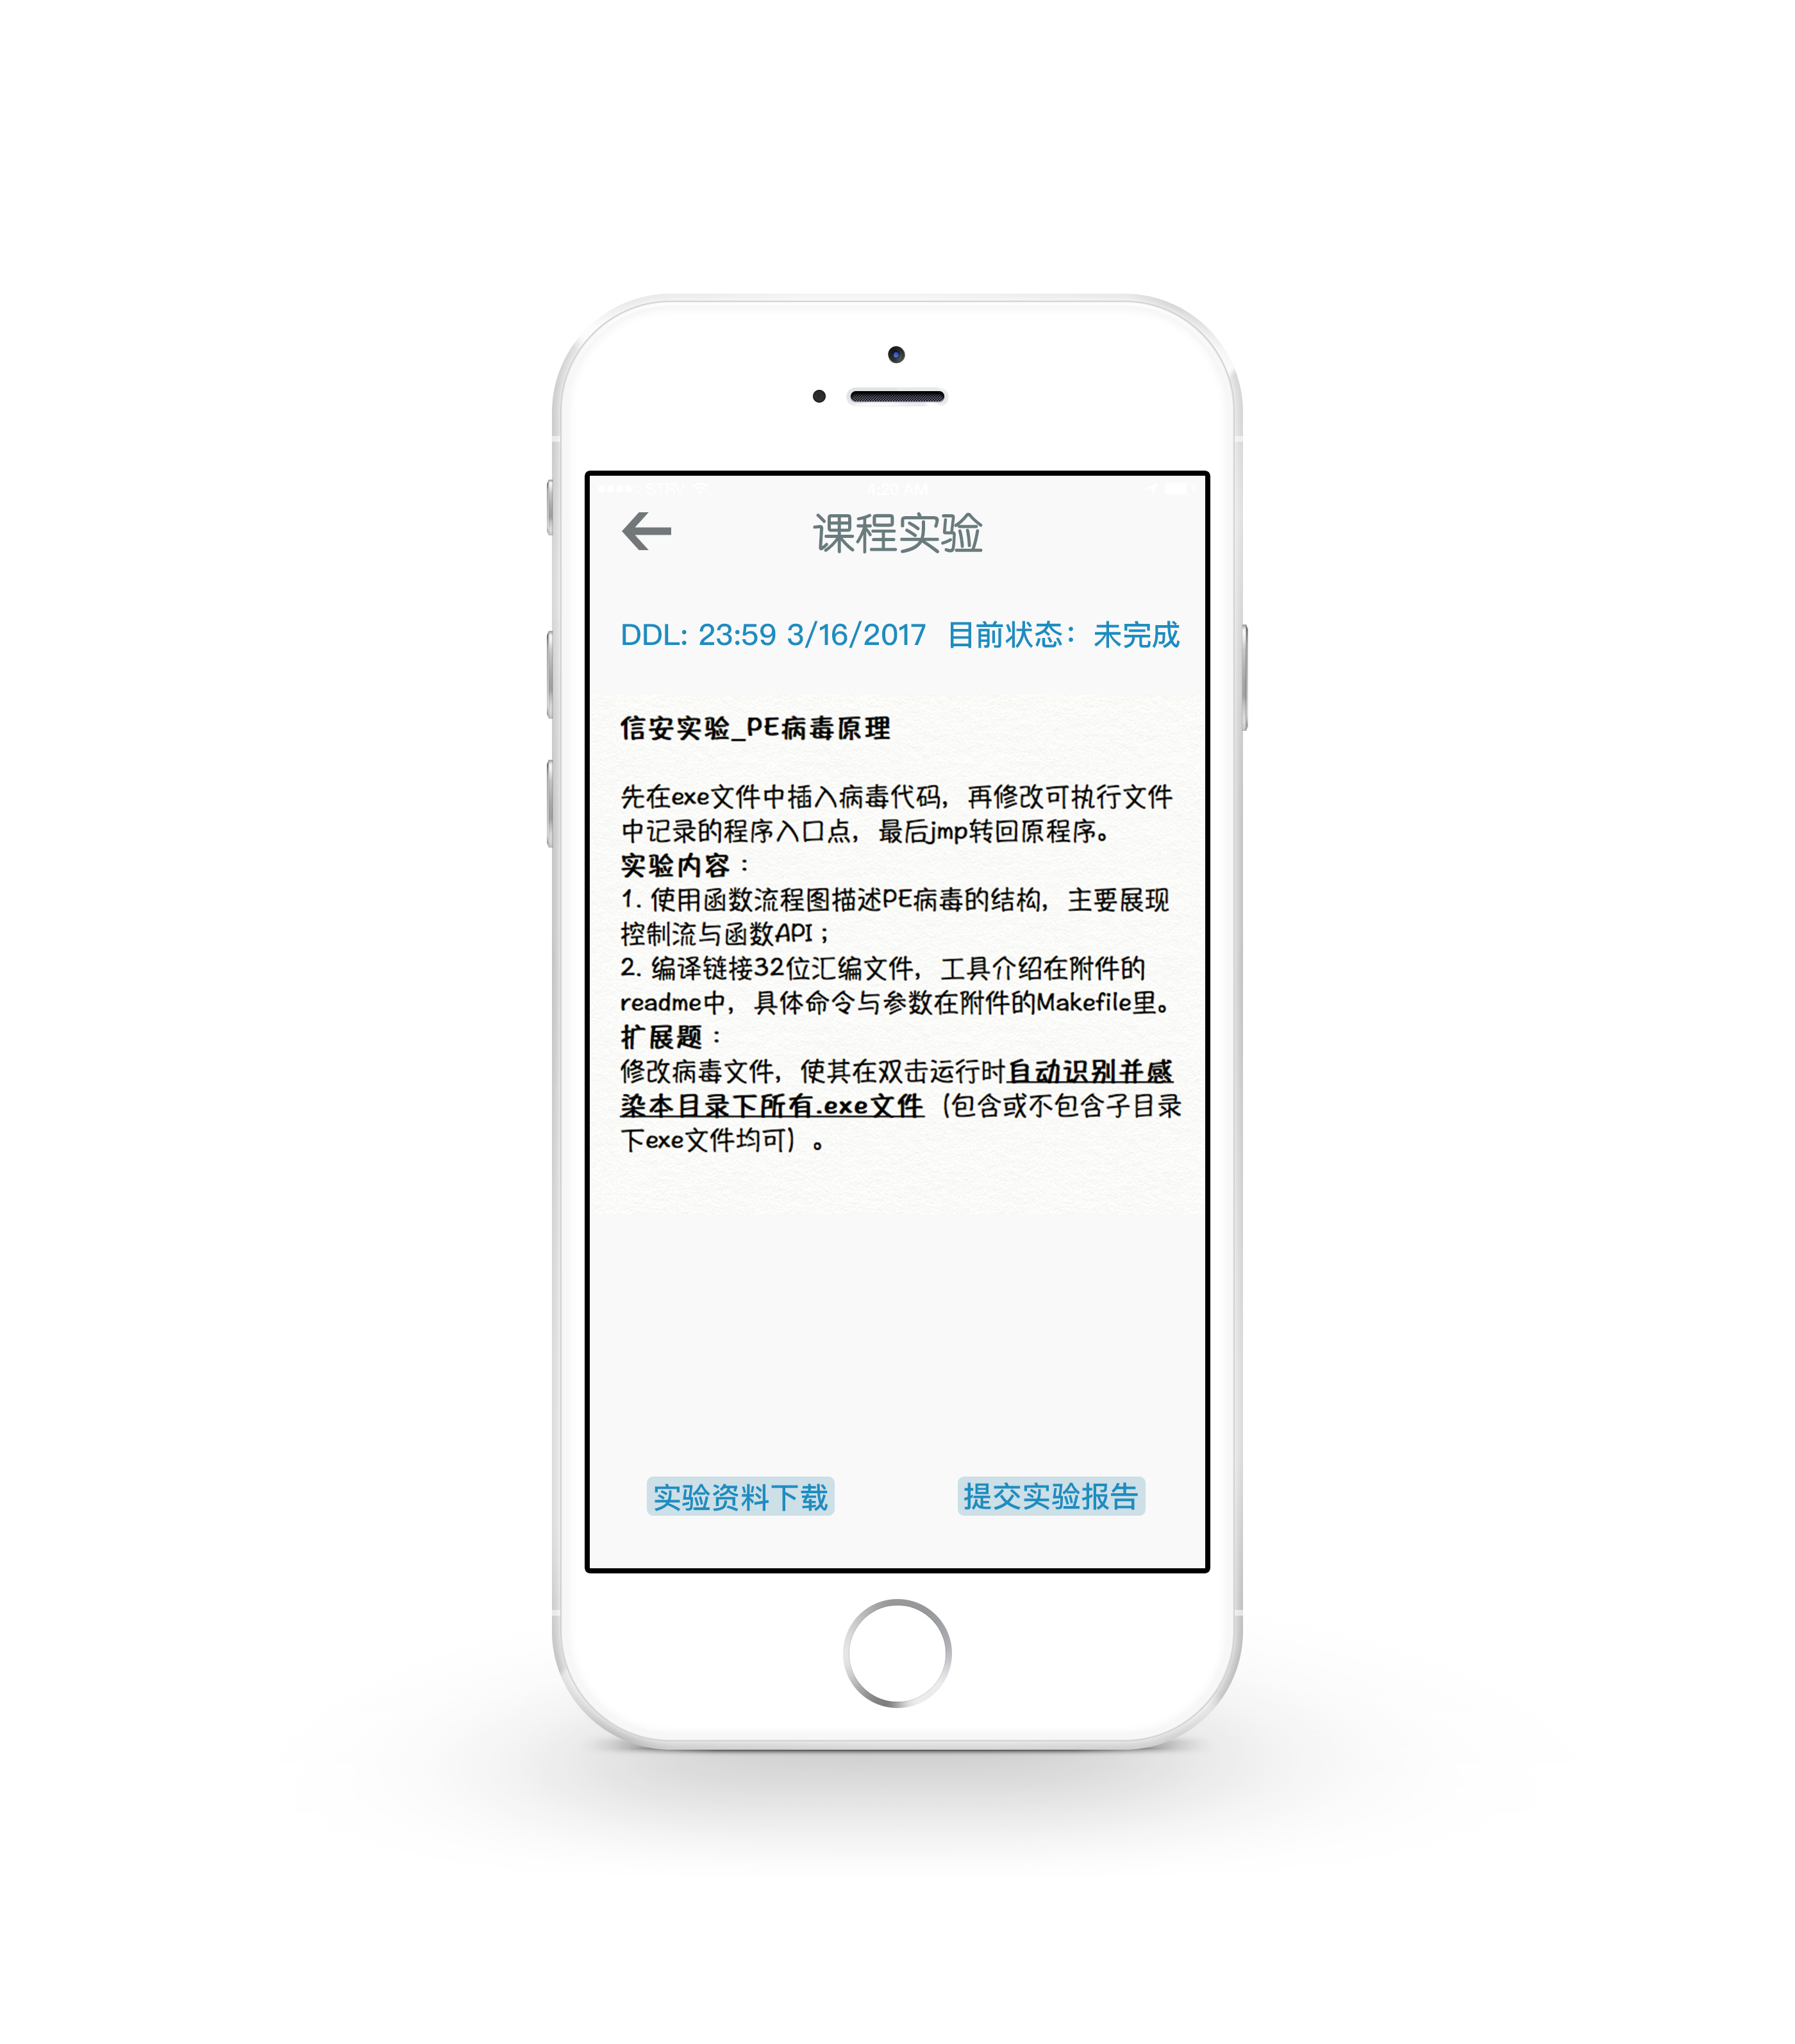
\includegraphics[width=10cm]{experiment_detail}
  \caption{实验详情}
  \end{figure}
  \item DDL:点击跳转到实验日期的日历显示界面
  \item 实验资料下载:下载本次实验的试验资料
  \item 提交实验报告:上传本地的实验报告
  \end{itemize}
  \subsubsection{R.HW.INTF.BB.004 讨论区}
    \begin{figure}[H]
    \centering
    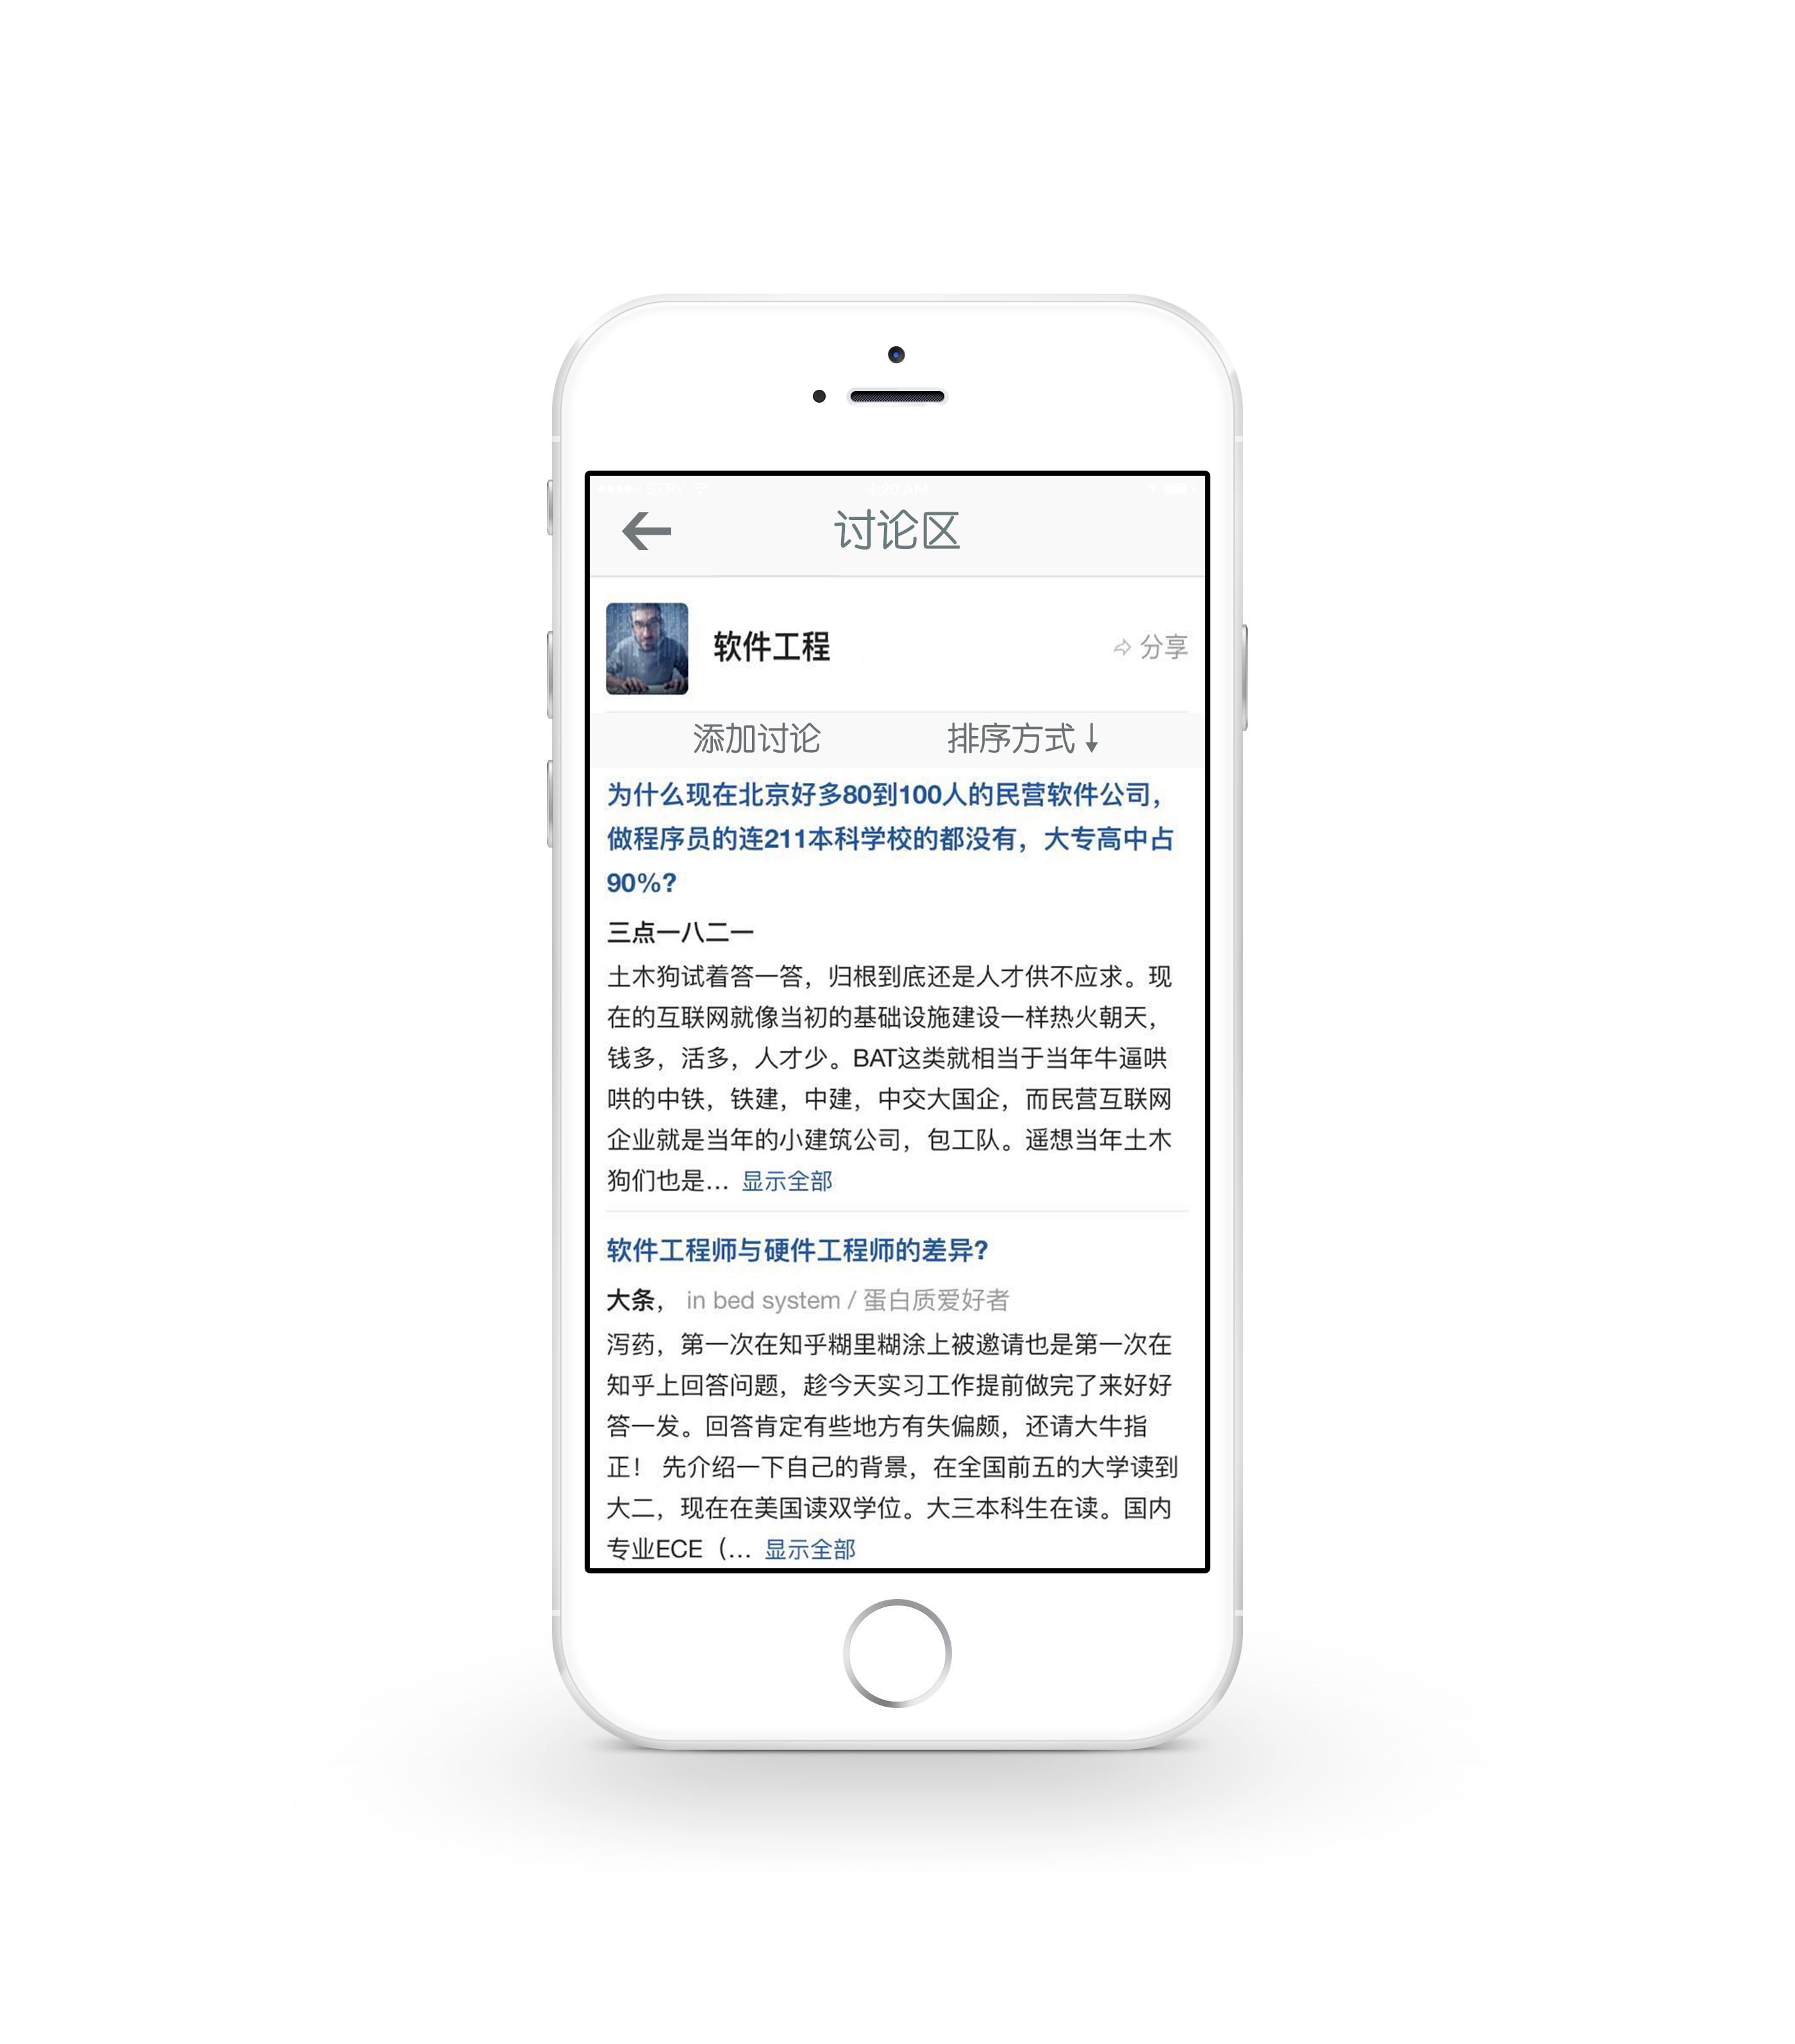
\includegraphics[width=10cm]{Discussion}
    \caption{讨论区}
    \end{figure}
  \begin{itemize}
  \item 分享:将课程讨论区分享给其他用户或其他软件
  \item 添加讨论:发布新的主题
  \item 排序方式:选择不同的排序方式
  \item 点击讨论主题标题:进入讨论主题详情
  \end{itemize}
  \subsubsection{R.HW.INTF.BB.005 笔记}
  \begin{figure}[H]
  \centering
  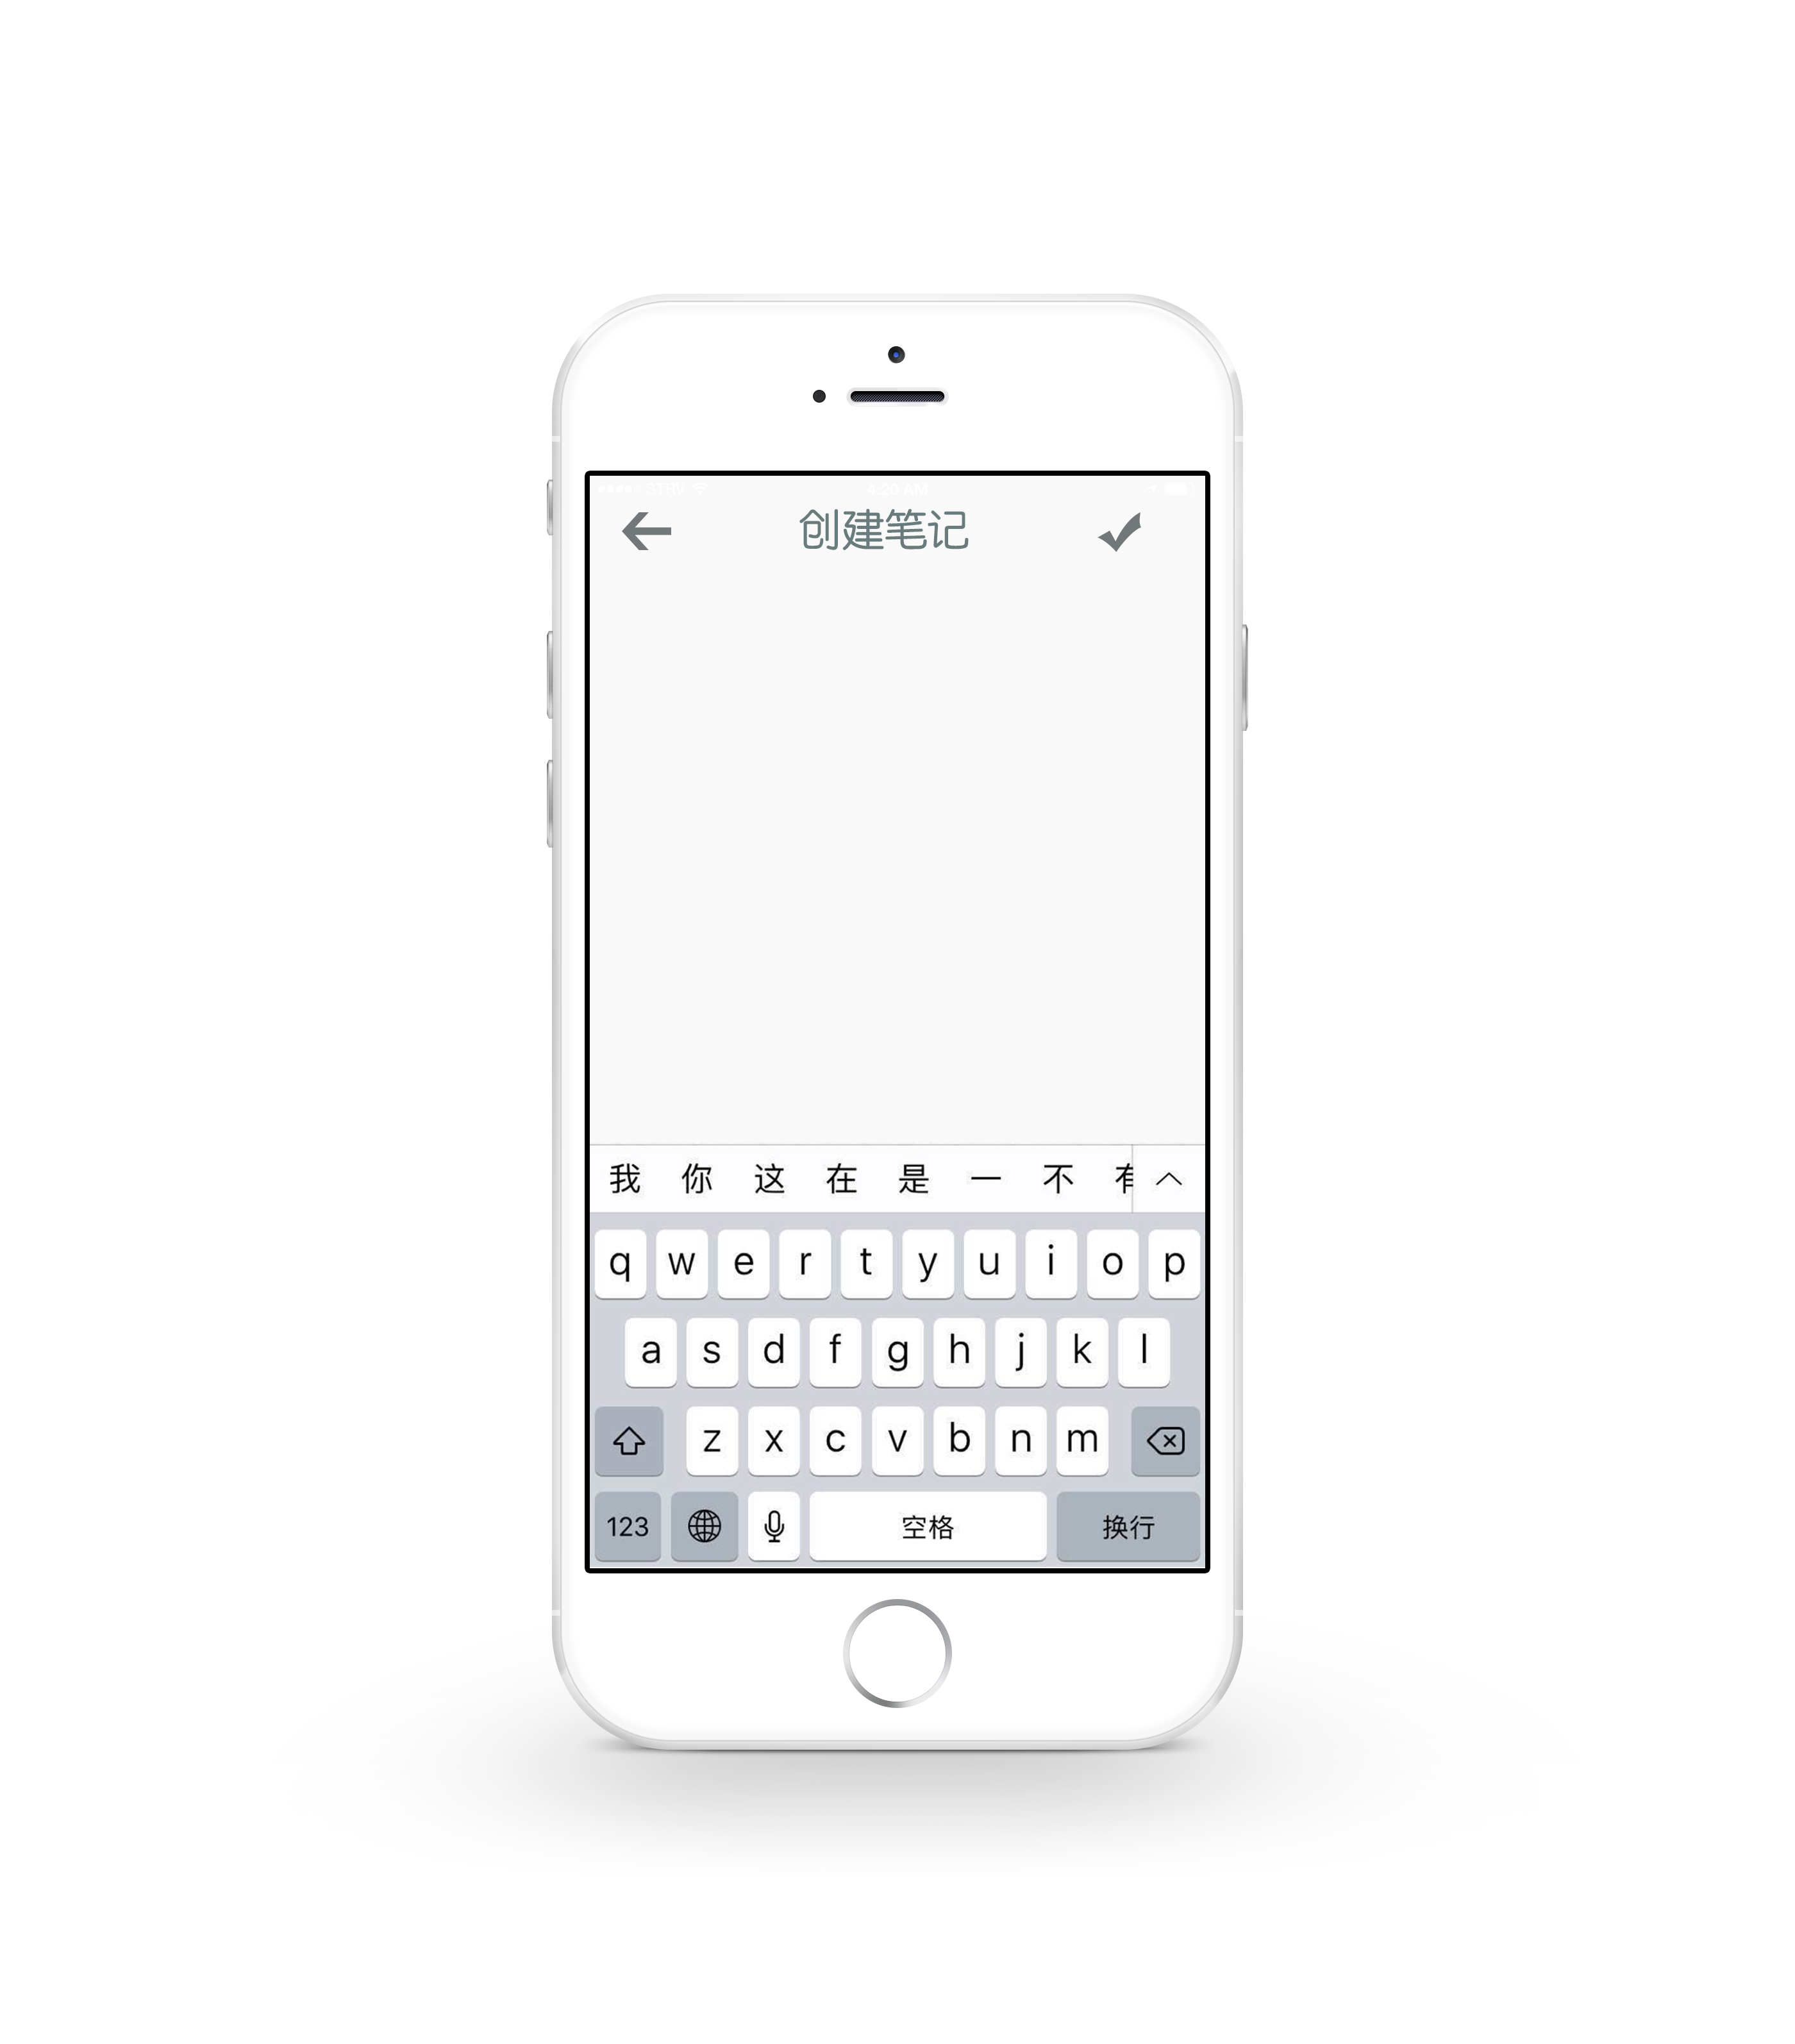
\includegraphics[width=10cm]{CreateNote}
  \caption{笔记编写}
  \end{figure}
  \begin{itemize}
  \item 返回按钮:退出编辑,返回上一级,不保存
  \item 笔记编写:键盘输入编写内容
  \item $\surd$ :编写玩笔记,保存并返回
  \end{itemize}

  \subsection{软件接口}
    \subsubsection{R.SW.INTF.BB.001 数据库}
	   \begin{center}\begin{description}
      \item[名称] Mysql数据库
      \item[助记符] Mysql
      \item[版本号]5.7.18
	     \item[来源] GPL
	      \item[接口] Database、Table相关操作和权限接口
	     \end{description}\end{center}

    \subsubsection{R.SW.INTF.BB.002 服务器系统}
	   \begin{center}\begin{description}
      \item[名称] macOS Sierra
      \item[助记符] OS
      \item[版本号] macOS Sierra 10.12.3
	     \item[来源] GPL
	      \item[接口] 服务器系统管理员权限和操作
	   \end{description}\end{center}

     \subsection{R.SW.INTF.BB.003 硬件接口}
     \subsubsection{Android系统}
	    \begin{center}\begin{description}
      \item[名称] Android操作系统
      \item[助记符] Android
      \item[版本号]
	\item[来源] Google
	\item[接口] App开发软件接口,硬件支持
	\end{description}\end{center}

    \subsubsection{R.SW.INTF.BB.004 iOS系统}
	\begin{center}\begin{description}
      \item[名称] iOS操作系统
      \item[助记符] iOS
      \item[版本号] iOS 10
	\item[来源] Apple
	\item[接口] App开发软件接口,硬件支持
	\end{description}\end{center}

  \subsection{通讯接口}
	TCP/IP网络服务
